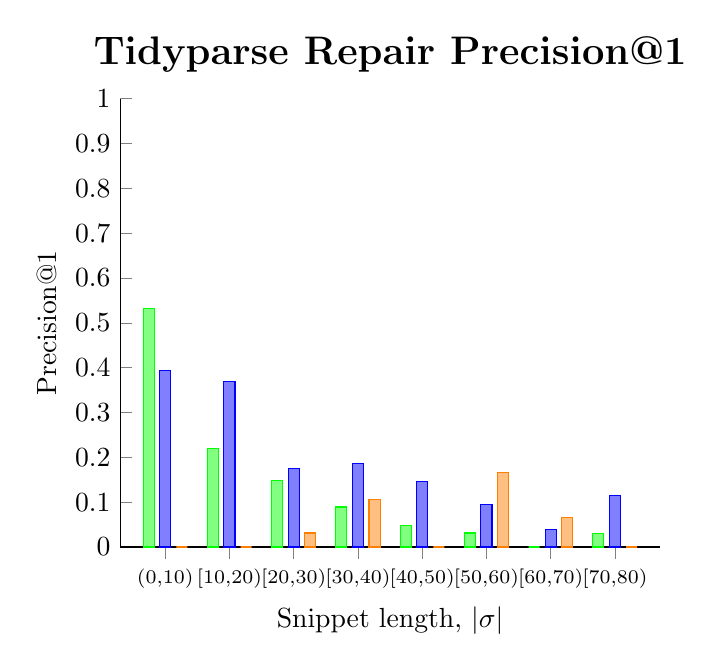
\begin{tikzpicture}
  \begin{axis}[
    xlabel={Snippet length, $|\sigma|$},
    ylabel={Precision@1},
    title={\Large\textbf{Tidyparse Repair Precision@1}},
    ybar,
    axis lines*=left,
    xtick={0, 10, 20, 30, 40, 50, 60, 70},
    ytick={0, 0.1, 0.2, 0.3, 0.4, 0.5, 0.6, 0.7, 0.8, 0.9, 1.0},
    xticklabels={{(}0{,}10{)}, {[}10{,}20{)}, {[}20{,}30{)}, {[}30{,}40{)}, {[}40{,}50{)}, {[}50{,}60{)}, {[}60{,}70{)}, {[}70{,}80{)}},
    x tick label style={font=\scriptsize},
    ymax=1.0,
    ymin=0.0,
    bar width=4pt,
  ]
%  \addplot[green, fill=green!50] coordinates { (0, 0.5) (10, 0.1827956989247312) (20, 0.08366533864541832) (30, 0.06572769953051644) (40, 0.016) (50, 0.020833333333333332) (60, 0.0) (70, 0.014705882352941176) };
%  \addplot[blue, fill=blue!50] coordinates { (0, 0.39285714285714285) (10, 0.42105263157894735) (20, 0.2037037037037037) (30, 0.20588235294117646) (40, 0.14666666666666667) (50, 0.06349206349206349) (60, 0.08) (70, 0.08571428571428572) };
%  \addplot[orange, fill=orange!50] coordinates { (0, 0.0) (10, 0.0) (20, 0.03125) (30, 0.10526315789473684) (40, 0.0) (50, 0.08333333333333333) (60, 0.06666666666666667) (70, 0.0) };
%  \addplot[green, fill=green!50] coordinates { (0, 1.0) (10, 1.0) (20, 1.0) (30, 1.0) (40, 1.0) (50, 1.0) (60, 1.0) (70, 1.0) };
%  \addplot[blue, fill=blue!50] coordinates { (0, 1.0) (10, 1.0) (20, 1.0) (30, 1.0) (40, 1.0) (50, 1.0) (60, 1.0) (70, 1.0) };
%  \addplot[orange, fill=orange!50] coordinates { (0, 0.25) (10, 0.14285714285714285) (20, 0.3125) (30, 0.42105263157894735) (40, 0.375) (50, 0.25) (60, 0.6) (70, 0.3333333333333333) };
  \addplot[green, fill=green!50] coordinates { (0, 0.53125) (10, 0.22043010752688172) (20, 0.14741035856573706) (30, 0.0892018779342723) (40, 0.048) (50, 0.03125) (60, 0.0) (70, 0.029411764705882353) };
  \addplot[blue, fill=blue!50] coordinates { (0, 0.39285714285714285) (10, 0.3684210526315789) (20, 0.17592592592592593) (30, 0.18627450980392157) (40, 0.14666666666666667) (50, 0.09523809523809523) (60, 0.04) (70, 0.11428571428571428) };
  \addplot[orange, fill=orange!50] coordinates { (0, 0.0) (10, 0.0) (20, 0.03125) (30, 0.10526315789473684) (40, 0.0) (50, 0.16666666666666666) (60, 0.06666666666666667) (70, 0.0) };
  \end{axis}
\end{tikzpicture}

%                                    TIDY-GWA                     TIDY-CFG                  TIDY-ENUM
%(|σ|∈[0, 10), Δ=1): Top-1/total:    56 / 100 = 0.56               54 / 99 = 0.55            57 / 100 = 0.57
%(|σ|∈[0, 10), Δ=2): Top-1/total:    37 / 100 = 0.37              19 / 100 = 0.19            22 / 100 = 0.22
%(|σ|∈[0, 10), Δ=3): Top-1/total:      9 / 50 = 0.18                6 / 50 = 0.12              6 / 50 = 0.12

%(|σ|∈[10, 20), Δ=1): Top-1/total:   44 / 100 = 0.44              42 / 100 = 0.42            45 / 100 = 0.45
%(|σ|∈[10, 20), Δ=2): Top-1/total:   28 / 100 = 0.28              13 / 100 = 0.13            14 / 100 = 0.14
%(|σ|∈[10, 20), Δ=3): Top-1/total:   20 / 100 = 0.20               9 / 100 = 0.09             8 / 100 = 0.08

%(|σ|∈[20, 30), Δ=1): Top-1/total:   43 / 100 = 0.43              49 / 100 = 0.49            49 / 100 = 0.49
%(|σ|∈[20, 30), Δ=2): Top-1/total:   26 / 100 = 0.26              13 / 100 = 0.13            18 / 100 = 0.18
%(|σ|∈[20, 30), Δ=3): Top-1/total:    19 / 99 = 0.19                8 / 99 = 0.08              8 / 99 = 0.08

%(|σ|∈[30, 40), Δ=1): Top-1/total:   49 / 100 = 0.49              43 / 100 = 0.43            48 / 100 = 0.48
%(|σ|∈[30, 40), Δ=2): Top-1/total:   24 / 100 = 0.24              15 / 100 = 0.15            18 / 100 = 0.18
%(|σ|∈[30, 40), Δ=3): Top-1/total:   15 / 100 = 0.15              10 / 100 = 0.10             6 / 100 = 0.06

%(|σ|∈[40, 50), Δ=1): Top-1/total:   55 / 100 = 0.55              56 / 100 = 0.56            57 / 100 = 0.57
%(|σ|∈[40, 50), Δ=2): Top-1/total:   19 / 100 = 0.19              21 / 100 = 0.21            18 / 100 = 0.18
%(|σ|∈[40, 50), Δ=3): Top-1/total:   10 / 100 = 0.10               8 / 100 = 0.08             5 / 100 = 0.05

%(|σ|∈[50, 60), Δ=1): Top-1/total:   55 / 100 = 0.55              67 / 100 = 0.67            53 / 100 = 0.53
%(|σ|∈[50, 60), Δ=2): Top-1/total:   25 / 100 = 0.25              16 / 100 = 0.16            21 / 100 = 0.21
%(|σ|∈[50, 60), Δ=3): Top-1/total:    9 / 100 = 0.09               9 / 100 = 0.09             7 / 100 = 0.07

%(|σ|∈[60, 70), Δ=1): Top-1/total:   53 / 100 = 0.53              56 / 100 = 0.56            60 / 100 = 0.60
%(|σ|∈[60, 70), Δ=2): Top-1/total:   23 / 100 = 0.23              15 / 100 = 0.15            10 / 100 = 0.10
%(|σ|∈[60, 70), Δ=3): Top-1/total:   11 / 100 = 0.11               5 / 100 = 0.05             2 / 100 = 0.02

%(|σ|∈[70, 80), Δ=1): Top-1/total:   57 / 100 = 0.57              62 / 100 = 0.62            63 / 100 = 0.63
%(|σ|∈[70, 80), Δ=2): Top-1/total:   18 / 100 = 0.18              12 / 100 = 0.12            15 / 100 = 0.15
%(|σ|∈[70, 80), Δ=3): Top-1/total:     9 / 81 = 0.11                4 / 81 = 0.05              3 / 81 = 0.04